\documentclass[a4paper,10pt]{article}

\usepackage{amssymb}%Blacksquare
\usepackage[margin=0.7in]{geometry}
\usepackage{amsmath,amssymb}
\usepackage{parskip,graphicx} 
\usepackage[makeroom]{cancel} %used to cross out terms in equations
\usepackage[utf8]{inputenc} %not clear effect
\usepackage[T1]{fontenc} %not clear effect
\usepackage[english]{babel}% not clear effect
\usepackage{float} %used for fixed tables with [H]

\floatstyle{plaintop} %used to place table caption on top
\restylefloat{table}

\usepackage[document]{ragged2e} %used to justify text
\usepackage{amsthm}
\usepackage{commath}
\usepackage{textcomp}
\usepackage{enumerate}
\usepackage{wrapfig}
\usepackage{epstopdf}
\usepackage{subfig}
\usepackage[font=small,labelfont=bf,
   justification=justified,
   format=plain]{caption}
\usepackage{array}% http://ctan.org/pkg/array	
\usepackage{breqn} %used to split equations on multiple lines
\usepackage{listings}
\usepackage{pdfpages} %used to include pdfs

\usepackage{siunitx} %used for units

\usepackage{titlesec}
\usepackage[titletoc,toc,title]{appendix} %used for apendix

\newcommand\numberthis{\addtocounter{equation}{1}\tag{\theequation}} %used for numbering only one equation 

\usepackage{braket} %quantum brackets
\DeclareMathAlphabet\mathbfcal{OMS}{cmsy}{b}{n}%caligraphy font

\numberwithin{equation}{section}

%used for pointing at equations
\usepackage{pst-node}
\usepackage{tikz-cd} 

\usepackage{tikz}
\usetikzlibrary{tikzmark}




\usepackage[nottoc]{tocbibind}

\usepackage{comment}
\usepackage{fancyhdr}

\newcommand{\parl}{\overset{\leftarrow}{\partial}}
\newcommand{\parr}{\overset{\rightarrow}{\partial}}

%used for boxing equations
\usepackage{empheq}
\usepackage{xcolor}
\definecolor{lightgreen}{HTML}{90EE90}
\newcommand{\boxedeq}[2]{\begin{empheq}[box={\fboxsep=6pt\fbox}]{align}\label{#1}#2\end{empheq}}

%used for disjoint unions
\newcommand{\cupdot}{\mathbin{\mathaccent\cdot\cup}}

\usepackage{tcolorbox}
\tcbuselibrary{theorems}

\newtcbtheorem{futwork}{Future work}%
{colback=white,colframe=white,coltitle=black,fonttitle=\bfseries}{fw}


\usepackage{hyperref} %Used to hyper reference.Usually it has to be the last package to be imported, but there might be some exceptions to this rule.

\pagestyle{fancy}
\fancyhf{}
\fancyhead[L]{\rightmark}
\fancyhead[R]{\thepage}
\renewcommand{\headrulewidth}{0.4pt}



\begin{document}
\pagenumbering{gobble}



\begin{titlepage}
 
\begin{center}
 
\begin{figure}[H]
\raggedleft
\includegraphics[width=0.3\linewidth]{jacobslogo.jpg}
\end{figure}
\LARGE
\text{Jacobs University Bremen} \\
\text{Department of Physics and Earth Sciences}
 
\vspace{25mm}
\huge{Quantization Procedures and the Time-Energy Uncertainty} \\
 
\vspace{15mm}
\Large{Project Thesis}\\
\vspace{2mm}
\large{as part of the course}\\
\vspace{2mm}
\large{CA08-200303 Project Physics}\\
\vspace{7.5mm}


\end{center}

 \begin{minipage}{0.4\textwidth}
\begin{flushleft} 
\textit{Author:} \\
\large{Daniel Prelipcean}

\end{flushleft}
\end{minipage}
\hfill
\begin{minipage}{0.4\textwidth}
\begin{flushright} 
\textit{Research Supervisor:} \\
\large Prof. Dr. Peter Schupp
\end{flushright}
\end{minipage}
 
 \begin{center}
\large{\textbf{\textsc{Abstract:}}}
\justify
Quantization procedures, in particular for constrained systems like the point particle, were investigated in order to derive and interpret the Time Energy Uncertainty Relation (TEUR). Two reviews, one of canonical quantization procedures and one of the TEUR, are presented. The canonical quantization of the free relativistic point particle is carried out in a general background, as well as deformation quantization in a static background. Future work includes obtaining uncertainty relations in deformation quantization and its generalization for some explicit metrics, as well as to investigate other minor inconsistencies in the canonical approach.
\end{center}
 
 \vfill
\begin{center}
\normalsize{\large{Bremen, \today}}
\end{center}
\end{titlepage}




\newpage

\setcounter{tocdepth}{3}
\tableofcontents

\newpage
\justify

\pagenumbering{arabic}
\setcounter{page}{1}

\section{Introduction: Motivation and Thesis Summary}

Rigorous formalism often comes only after the discovery process, and not during or before. A mistery still standing is the derivation and interpretation of the Heisenberg time-energy uncertainty relations. Compared to the the position and momenta uncertainty relations, they lack a solid mathematical derivation. However, it is may be possible that we understand a theory perfectly well physically, that mathematical rigour is an unnecessary luxury. Nevertheless, I take the view that there exists a clear structure beneath the variety of heuristic notions physicists use when approaching and understanding physical phenomena. And while any physical theory is necessarily an approximation, the structure of the theory need not be “approximate.”


Since the introduction of the uncertainty relation between position and momenta operators \cite{HeisenbergUR}, a controversial issue were the time-energy commutation relations:
\begin{equation}
    Et - tE = -i\hbar \qquad \text{or} \qquad  Jw - wJ = -i\hbar
\end{equation}
which would give the time-energy uncertainty relations (TEUR):
\begin{equation}
    \Delta E \Delta t \geq \hbar/2 \qquad \text{or} \qquad  \Delta J \Delta w \geq \hbar/2
\end{equation}


where $J$ is the action variable and $w$ is the angle variable (a time indicating coordinate in perdiodical motion). This already introduced confusion as one noted in Ref. \cite{BuschTEUR}, since: i) it suggests the existence of a time operator and ii) it mixes up energy and time with action and angle variables. Different types of TEUR do indeed hold depending on the context (interpretation of what time means), in spite of some Gedankenexperiments like Einstein`s photon box. However, a unique universal TEUR similar to the position-momentum does not exist in the standard view of QM.

In relativistic QM, where time promoted to a canonical variable with the Hamiltonian as conjugated momentum, the canonical TEUR \cite{HeisenbergUR} holds axiomatically as:
\begin{equation}
    \Delta T \cdot \Delta E \geq \frac{\hbar}{2}
\end{equation}
In doing so, a new parameter time evolution has to be introduced and, depending on the gauge fixing, it may be identical to the original coordinate time, possibly rendering the above relation futile. In any case, further interpretation of the time energy relation is needed.

This thesis is organized as follows. Section \ref{sec:TimeQgrav} presents a short review of the problem of time in combining Quantum Mechanics and General Relativity. Section \ref{sec:relaprticleaction} shows how even the most simple state (a single particle in a gravitational background) implies a static universe. The new work of this thesis is presented in section \ref{sec:staticworldinterpretation}, where a novel interpretation to the mass-shell condition is given. Further discussion, results and future outlook are given in section \ref{sec:discussion}.

\newpage
\section{The Problem of Time in Quantum Gravity}
\label{sec:TimeQgrav}

Quantization is the transition from the classical analysis of physical phenomena to a newer understanding known as quantum mechanics, and thus it is the procedure for building quantum mechanics \textit{from} classical mechanics. Considering that the world is truly quantum and the everyday world represents the "classical" limit, one finds that the quantization process is not unique, i.e. one needs to add several concepts and can do so along different paths.
The three logically sound paths to quantization developed so far are:
\begin{enumerate}
    \item  
The Canonical Quantization Procedure, which attempts also to preserve the formal structure of the classical theory, to the greatest extent possible. 

\item 
Path Integrals, conceived by Dirac and developed by Feynmann, involving a functional integral over all topologically allowed trajectories to compute a quantum amplitude.

\item
Deformation Quantization or Phase-Space Formulation, based on Wigner's quasi-distribution function and Weyl's correspondence between quantum-mechanical operators and ordinary phase-space functions.
\end{enumerate}

Different approaches to combine Quantum Mechanics (QM) with General Relativity (GR) have been made, but the "Holy Grail" of Theoretical Physics is yet to be found. The first immediate issue is the Problem of Time, which occurs because \textit{time} takes a different meaning in each of QM and GR. A quite philosophical review of this question is presented in Ref. \cite{AndersonTimeQG}.


\begin{figure}[H]
    \centering
    
\[ \begin{tikzcd}
\mathcal{L} \arrow{r}{LT} & H \arrow{r}{Quant.} \arrow[swap]{d}{Red.} & \hat{H} \arrow{d}{Red.} \\%
& \tilde{H} \arrow{r}{Quant.}&  \tilde{\hat{H}}
\end{tikzcd}
\]
    \caption{The usual starting point is the Lagrangian $\mathcal{L}$, whence one derives the Hamiltonian $H$ via a Legendre Transformation (LT). Next, Quantization and Reduction to the physical phase-space (for constrained systems) have to be performed. The question, which now arises, is whether Quantization and Reduction commute or not. This is yet to be fully answered. Moreover, the Legendre transformation itself may impose problems.}
    \label{quantizationscheme}
\end{figure}



\subsection{Canonical Quantization and Explicit Quantization Schemes}
The Canonical approach is inspired from the Hamiltonian approach to classical mechanics, in which a system's dynamics is generated via canonical Poisson brackets. However, not all properties are preserved. The Canonical approach to Quantum Mechanics can be summarized by asserting that the classical Poisson brackets are replaced by commutators. Mathematically, this represents finding a quantization map $Q$ such that any function on the classical phase-space gets promoted to an operator $\hat{Q}_f$:
\begin{equation}
    \{Q_f,Q_g\} \rightarrow \frac{1}{i\hbar} [ \hat{Q}_f, \hat{Q}_g ]
\end{equation}
The following properties are desirable \cite{Qproperties} for the quantization map $Q$ :
\begin{enumerate}
    \item Position and momentum representation, e.g. $\hat{Q}_x \psi = x \psi$ and   $\hat{Q}_p \psi = - i \hbar \partial_x \psi$
    
    \item Linearity of $f \stackrel{Q}{\rightarrow} \hat{Q}_f$
    
    \item Poisson brackets: $i\hbar Q_{\{f,g\}} = [ \hat{Q}_f, \hat{Q}_g ]$
    
    \item von Neumann rule: $Q_{\{g \circ f\}} = g(Q_f)$
\end{enumerate}


Unfortunately, these four properties are mutually inconsistent \cite{incompatibility}. Just as one example of this incompatibility, Groenewold`s theorem states that there is no such quantization map $Q$ on polynomials of degree less than or equal to four whenever $f$ and $g$ have degrees less than or equal to three.

The only pair of these properties that lead to self-consistent, nontrivial solutions are two (2) and three (3). Hence, there is \textit{no} such quantization map satisfying the above.  In particular, accepting the first two properties and a weaker condition of the third one (to be true only asymptotically in the limit $\hbar \to 0$, yielding Moyal brackets), leads to deformation quantization, tackled later in this paper.



\begin{enumerate}

\item 
Dirac Quantization \cite{DiracQMLectures}: The classical Poisson Bracket is altered to implement system's constraints $\psi_j$ with Lagrange multipliers $u_j$. Given initial $k$ constraints $\psi_j$, with $j = 1$ to k, one has to iteratively find all subsequent constraints obeying the consistency condition:
\begin{equation}
    \dot{\psi_j} = \{H, \psi_j \} + \sum_{i\neq j}^k u_i \{\psi_j, \psi_i \} 
\end{equation}
This condition may give rise to new constraints $\psi_j$, with $j>k$. The procedure ends when no new constraints (that cannot be expressed as previous constraints) are found. All constrainsts are then further classified into:
\begin{enumerate}
\item First class if their Poisson brackets vanish on the constraint surface defined by $C_\alpha (z) = 0$:
\begin{equation}
\{ C_\alpha, C_\beta \} = f_{\alpha \beta}^\gamma C_\gamma
\end{equation}

\item Second class, if their Poisson brackets do not vanish on their constraint surface:
\begin{equation}
det\{\chi_a, \chi_b\}|_{\chi_a = 0} \neq 0
\end{equation}
\end{enumerate}
The improved Poisson brackets are called Dirac brackets:
\begin{equation}
    \{F, G\}_{D} = \{F, G \}_{PB} - \{F, \chi_m\} \Lambda^{mn}\{\chi_n, G\}
\end{equation}
where $\Lambda^{mn} = det\{\chi_m, \chi_n\}$.



\item 
BRST-BV Quantization \cite{BRSTprimer, BVformalism}: The constraints are promoted to another first-order object, accomplished by extending the target space F by a Grassmann algebra of “ghost-antighost pairs,” while maintaining its structure as a symplectic manifold. That is, the cotangent bundle is promoted to a super-Poisson manifold, whose odd coordinates are given by the ghost-antighost pairs. This procedure is mainly used for gauge-invariant theories.


\item 
Fadeev-Jackiw Quantization \cite{withouttears}: It can be considered as an alternative shorter Dirac version of quantization for certain scenarios. It implies reaching the desired formulas for brackets and for the Hamiltonian even for constrained Lagrangians, and it is based on Darboux`s theorem. In particular, it is used when the Lagrangian depends linearly on velocities, and one does not need to distinguish between first and second class constraints.

\end{enumerate}








\subsection{Time in Classical Mechanics}


In the Lagrangian-Hamiltonian formalism, one would like to extend the $(2n)$ dimensional phase space $T^*M$, locally defined by pairs $\{(x; p)\}$, by introducing energy and time as the $(n + 1)$ canonical conjugate pair, to finally reach a relativistically covariant description. However, this program cannot be carried through, i.e. it is not possible to find a Hamiltonian that generates the motion in the enlarged phase space \cite{JanNoTimeCoordinate}. The first intuitive problem is already the fact the H is not independent of the other canonical variables. 

Treating time $t = q_0$ completely symmetrically with the others, one can obtain a symmetric Lagrangian, that is, promoting time to a canonical coordinate and introducing some other evolution parameter $\tau$, which is any arbitrary, continuous parameter that varies monotonically and differentiably along the path of the motion of the Lagrangian in the tangent bundle $TM$, locally defined by pairs$\{(q_i; \dot{q}_i)\}$, with $i = 0$ to $N$. Introducing a "unified variational principle", one obtains the Lagrange equations of motion for all coordinates $(q_i)$, with $i = 0$ to $N$, together with a dependence relation (or constraint) of the form $f(q_i) = 0$. This implies that the Legendre transform $L(q_i, \dot{q}_i) \rightarrow H(q_i, p_i)$ cannot be performed.


However, the Hamiltonian equations can be obtained if one sets any pair of the $(n + 1)$  phase-space variables $(q, p)$ from the list of canonical variables to serve as a system parameter, replacing the evolution parameter $\tau$.


\iffalse
A general class of 'timelike' canonical variable is formed by the angle variables (e.g. defining the direction of the hands of a clock), with corresponding canonical momenta called action variables, such that the Hamiltonian takes the form $H = H(J1; :::; Jn)$, i.e. does not depend on the angle variables.
\fi

\subsection{Reparametrization Invariance and Static World}
\label{frozenintime}.

It is shown in Ref. \cite{noHamiltonian} that there is no definition of a symmetric (that is, treating time on equal footing with space) non-vanishing Hamiltonian $H(q_i, p_i)$ for which the Hamiltonian equations:

\begin{equation}
    \dot{q}_i = \frac{\partial H(q_i,p_i) }{\partial p_i} \qquad \text{and} \qquad  \dot{p}_i = - \frac{\partial H(q_i,p_i) }{\partial q_i}
\end{equation}

with $i = 0$ to $N$ are correct for any arbitrary choice of parameter $\tau$ and equivalent to the Lagrangian equations. The main aspect of the above result is that the desired Hamiltonian $H$ derived by a Legendre transformation is identically zero. Moreover, although it is possible in Lagrangian mechanics that a function that is constant on the unvaried path will still lead to useful differential equations because its variation $\delta H \neq 0$ is non-zero, this is not the case for our Hamiltonian $H$.

Moreover, quantizing the result of Section \ref{particleHamiltonian} implies a stationary, timeless equation:
\begin{equation}
    i \frac{\partial \psi}{\partial \tau} = \hat{H} \psi = 0
\end{equation}
In the case of GR, this is the Wheeler-De Witt equation \cite{WdWeq}, which occurs for any reparametrization invariant theory in a covariant approach. Alternatively, one may think that the vanishing Hamiltonian may imply that one is obliged to work in the Heisenberg picture of quantum mechanics, where time evolution appears in the operators. It would be surprinsingly beautiful, if one could define a time operator (not as imply as $\exp{( -iEt/\hbar)}$ that could be inserted into all other operators.



\subsection{Time in Quantum Mechanics}
Two opposite (mathematical) views of time in QM have appeared.  

\begin{enumerate}
    \item 
    Time is just a scalar, a parametric label for dynamical evolution. This is asserted in standard textbooks, e.g. by Sakurai: “The first important point we should keep in mind is that time is just a parameter in quantum mechanics, not an operator. In particular, time is not an observable. It is nonsensical to talk about the time operator in the same sense as we talk about the position operator." \cite{SakuraiQM}
    
    \item
   Time is indeed an operator and defining it is a difficult task. Von Neumann argued that the scalar view of QM is its main weakness: "First of all we must admit that this objection [time being just a number] points at an essential weakness, which is, in fact, the chief weakness of quantum mechanics." \cite{NeumannQM}
\end{enumerate}

Promoting time to a canonical coordinate, one then requires an extra evolution parameter for the respective system. Henceforth, the \textit{physical time} shall refer to the coordinate time, which gets promoted to an operator, and \textit{parameter time} shall refer to the evolution parameter of the system, which indeed is just a scalar. Therefore, both views of time are reconciled.

A further classification of time in non-relativistic quantum theory can be done, according to Ref. \cite{BuschTEUR}:
\begin{enumerate}
    \item \textit{external time:} Identified as the parameter entering the Schrödinger equation and measured by an external, detached laboratory clock. Such external time measurement are carried with clocks that are not dynamically connected to the quantum system
    
    \item \textit{intrinsic time:} As the dynamical evolution parameter $\tau_\phi(A)$ through which quantum observables $A$ change, giving a quantitative measure of the length of the time interval between two events
    
    \item \textit{observable time:} Promoting time to a quantum operator. 
    
\end{enumerate}

One already notices that the \textit{observable time} and the \textit{physical time} have the same philosophical meaning in the covariant quantum gravity language. Such confusion arises also due to mixing up the canonical position coordinates of a point particle and the coordinates of a point in space. In Ref. \cite{JanNoTimeCoordinate}, it is argued that there is no reason why coordinate time should be an operator in quantum mechanics.

A possible way to distinguish between intrinsic and observable time would be to define intrinsic time as: The time from which the quantum phenomenon under observation has started and it possibly finishes at decoherence. 


\subsection{Time Operators}

Considering time as an observable is motivated by the experiments in which times of events are recorded using lab clocks. The question is how one can relate this observed time with the intrinsic time of quantum phenomenon. In this paper, the parametric view of time does not suffice, as the main interest is the Time Energy Uncertainty Relation, which requires an operator interpretation of time. 

Quite early in the development of Quantum Mechanics, Pauli has argued that the existence of a self-adjoint time operator canonically conjugate with a Hamiltonian implies that both operators have continuous spectra spanning the entire real line, a result widely known as Pauli’s theorem \cite{pauli1980general}. This had a severe impact on the Hamiltonian of physical systems, which usually have a stable ground state (hence semi-bounded) or discrete (e.g. Harmonic Oscillator) since the time operator would not exist. 

Although Pauli`s theorem states that one cannot find a self-adjoint operator yielding time, for special cases (Hamiltonians) one can obtain such an operator, canonically conjugate to the hamiltonian, e.g. for a free falling particle \cite{BuschTEUR}:
\begin{equation}
    \hat{H}_g = \frac{\hat{P}^2}{2m} - mg\hat{Q} \Rightarrow \hat{T}_g = -\frac{1}{mg}\hat{P}
\end{equation}

Sticking with the Hilbert space formulation, it is considered that a compromise has to be made \cite{GalaponCanonicalPairs}.
\begin{enumerate}
    \item Imposing self-adjointness leads to violation of the Canonical Commutation Relations (CCR) with the Hamiltonian
    
    \item Strictly obeying the CCR leads to the proper time operator to not be self-adjoint
\end{enumerate}

Recently, the later route has been taken. This has also implied that the quantum observables have been extended to maximally symmetric bot not necessarily self-adjoing operators, i.e. generally positive operator valued measures (POVM). Defining a time observable through a POVM rather than a self-adjoint or symmetric operator was investigated by Brunetti and Fredenhagen \cite{Fredenhagen}, who performed normalization at the operator level. 

A further results \cite{galaponcanonicaltriple} states that a pair of Hilbert space operators $(Q, P)$ obeying the CCR can at most satisfy the CCR in a \textit{proper} subspace $\mathcal{D}_c \subset \mathcal{H}$. Therefore, a canonical-pair in a Hilbert space is a triple $\mathcal{C}\left( Q,P; \mathcal{D}_c\right)$. 

The relation between $\mathcal{D}_c$ and the reduced (constrained) phase space may not be trivial. Therefore, futher work may include investigating whether the subset $\mathcal{D}_c \subset \mathcal{H}$ coincides identically with the space of physical wavefunctions obeying the physical constraints (e.g. mass-shell condition).

In the free non-relativistic particle case, the Hamiltonian and its conjugate time operator are:
\begin{equation}
    H_{free} = \frac{P^2}{2m} \Rightarrow T = m\frac{q}{p}
\end{equation}

Quantizing, one has to consider the ordering of operators, and thus more symmetric terms are proposed, such as the Aharanov-Bohm's time operator:
\begin{equation}
T = m \dfrac{q}{p} \Rightarrow \qquad \hat{T} = \dfrac{1}{2}m \left( \hat{q}\hat{p}^{-1} + \hat{p}^{-1}\hat{q}\right) \qquad \text{ or} \qquad \hat{T} = \dfrac{m}{2} \left( \hat{p}^{-1/2} \hat{x} \hat{p}^{-1/2} \right)
\end{equation}

One can try to obtain a self-adjoint operator by using a formal series expansion, but runs into convergence problems (see Appendix \ref{timeoperatorconvproblems}). For the Hamiltonian of section \ref{particleHamiltonian}, the time operator before quantization for constant einbein and metric is:
\begin{equation}
T = \frac{1}{e} \frac{q}{p} \Rightarrow \hat{T} = \frac{1}{2}m \left( \hat{q} \hat{p}^{-1} + \hat{p}^{-1}\hat{q} \right)
\label{constanttimeoperator}
\end{equation}

\newpage


\section{The relativistic particle action}

\label{sec:relaprticleaction}

By introducing the einbein as an auxiliary field $e$ (See Appendix \ref{einbeinexplained}), one allows the action for massless particles to be non-trivial, namely:
\begin{equation}
    S = -\int d\lambda L = \int d\lambda \frac{1}{2} \left(\frac{1}{e} \dot{X}^{\mu}\dot{X}^{\nu}g_{\mu \nu} - e m^2 \right)
    \label{action}
\end{equation}

The evolution parameter $\lambda$ is not a measure of proper time for the particle unless the tangent vector is of unit length, i.e. $\dot{X}^\mu \dot{X}_\mu =1$. Any such parametrization will work, since the action $S$ is reparametrization invariant.

The einbein $e$ is considered to be an arbitrary function of the time evolution parameter $\lambda$, i.e. $e = e(\lambda)$ as a world-line reparametrization or equivalently as shorthand notation for $\sqrt{-\dot{X}^{\mu}\dot{X}^{\nu}g_{\mu \nu}}/m$. It is a non-dynamical function, like $p_\mu$, since $\dot{e}$ does not appeard in the action. For simplicity, the metric $g_{\mu \nu} = g_{\mu \nu}(X)$ was later particularized for the constant Minkowski metric $\eta_{\mu\nu} = diag(-,+,+,+)$.

\subsection{Equations of Motion}
The Lagrange equations of motion become:
\begin{subequations}
\begin{eqnarray}
    & p_\alpha  = \frac{\partial L}{\partial \dot{X}^\alpha} = \frac{1}{e} \dot{X}^{\mu}g_{\alpha \mu}
    \label{generalizedmomentum}  \qquad \dfrac{\partial L}{\partial X^\alpha} = \dfrac{1}{2e}\dot{X}^\mu \dot{X}^\nu \partial_\alpha g_{\mu\nu}
\\
    & \dfrac{\partial}{\partial \lambda}\left( \dfrac{\partial L}{\partial \dot{X}^\alpha}\right)  - \dfrac{\partial L}{\partial X^\alpha}  =  -\dfrac{\dot{e}}{e^2}\dot{X}^\nu g_{\alpha \nu} + \dfrac{1}{e}\ddot{X}^\mu g_{\alpha \mu} + \frac{1}{e}\dot{X}^\nu \dot{X}^\mu \partial_\nu g_{\alpha \mu} - \dfrac{1}{2e}\dot{X}^\mu \dot{X}^\nu \partial_\alpha g_{\mu \nu} = 0
\end{eqnarray}
\end{subequations}

One can obtain the Christoffel symbol from the last two terms, namely:
\begin{equation}
    \partial_\nu g_{\alpha \mu} - \frac{1}{2}\partial_\alpha g_{\mu \nu} = \frac{1}{2} \left( \partial_\nu g_{\alpha \mu} + \partial_\mu g_{\alpha \nu} - \partial_\alpha g_{\mu \nu} \right) = \Gamma_{\alpha \nu \mu}
\end{equation}

Raising the $\alpha$ index by multiplication with $g^{\alpha \nu}$ finally gives:
\begin{equation}
    \frac{1}{e}\left(\frac{-\dot{e}}{e}\dot{X}^\alpha + \ddot{X}^\alpha + \Gamma^\alpha_{\mu \nu} \dot{X}^\mu \dot{X}^\nu\right) = 0
\end{equation}

which is the geodesic equation for an affine parameter with the extra first term. Moreover, considering this parameter $\lambda$ as a general function of the proper time $\tau$, this relation becomes:
\begin{equation}
    \frac{-1}{e}\frac{de}{d\lambda}\frac{dX^\alpha}{d\lambda} + \frac{d^2X^\alpha}{d\lambda^2} + \Gamma^\alpha_{\mu \nu}\frac{dX^\mu}{d\lambda}\frac{dX^\nu}{d\lambda} = - \left(\frac{d^2 \lambda}{d\tau^2} \right)\cdot \left(\frac{d\lambda}{d\tau} \right)^{-2}\cdot\frac{dx^\alpha}{d\tau}
\end{equation}


An attempt to treat $e = e(X^{\mu},\lambda)$ and $ g_{\mu \nu}(X,\lambda,e)$ as general functions has also been carried out. Next to having close to no physical interpretation, no meaningful results were obtained.





\subsection{A word on the mass-shell constraint}

Varying this action with respect to $e$ yields its equation of motion:
\begin{equation}
    \frac{1}{e^2} \dot{X}^{\mu}\dot{X}^{\nu}g_{\mu \nu} + m^2 =0
    \label{alleom}
\end{equation}
Using the momenta definition of \ref{generalizedmomentum}, one obtains the mass-shell constraint $p_\mu p^\mu + m^2 = 0$ that we will indeed treat as an equation of motion. The Hamiltonian defined via Legendre Transform becomes:
\begin{equation}
    H = p_\mu \dot{X}^\mu - L = \frac{1}{2}e(p_\mu p^\mu + m^2) = 0
    \label{simpleHamiltonian}
\end{equation}

that is, an exactly vanishing Hamiltonian via the einbein equation of motion. The einbein thus introduced enforces the mass-shell condition, which shall be treated as a constraint weakly equal to 0, rather than an equation of motion exactly zero. The quantization of this result has been considered so far to yield the usual problem of time in quantum gravity, $\hat{H} \ket{\psi} = 0$.

One observes that this constraint is not linear in velocities (and not even semi-holonomic). This brings up the subtle issues of Hamiltonian mechanics not being able to deal with non-holonomic constraints (e.g. cannot be simply added by introducing Lagrange multipliers). A further topic to be investigated is the relation between Dirac constraints as First and Second Class with Holonomic and Non-Holonomic constraints.








\iffalse
\subsubsection{General metric}

An interesting case arises if one keeps a metric that explicitly depends on the einbein, i.e. $g_{\mu \nu} = g_{\mu \nu}(e, X^\alpha, \tau)$. The einbein equation of motion REF can be rewritten as:
\begin{equation}
    \frac{1}{e^2}\dot{X}^\mu \dot{X}^\nu g_{\mu \nu} + m^2 = - \frac{1}{e}\dot{X}^\mu \dot{X}^\nu \frac{\partial g_{\mu \nu}}{\partial e}
\end{equation}

Using this in the above formalism allows one to use Leibniz rule for chain derivatives, namely:
\begin{equation}
    \frac{\partial e}{\partial X^\alpha} \frac{\partial g_{\mu \nu}}{\partial e} = \frac{\partial g_{\mu \nu}}{\partial X^\alpha}
\end{equation}

Then, the coordinates derivatives surprisingly vanish:
\begin{equation}
    \frac{\partial L}{\partial X^\alpha } = \frac{1}{2e}\dot{X}^\mu \dot{X}^\nu \partial_\alpha g_{\mu \nu} - \frac{\partial e}{\partial X^\alpha } \frac{\partial g_{\mu \nu}}{\partial e}\frac{1}{2e}\dot{X}^\mu \dot{X}^\nu = \frac{1}{2e}\dot{X}^\mu \dot{X}^\nu \partial_\alpha g_{\mu \nu} - \frac{1}{2e}\dot{X}^\mu \dot{X}^\nu \partial_\alpha g_{\mu \nu} = 0
\end{equation}

This interestingly implies that the momenta are always constant in this scenario, regardless of the metric in questions (constant or not):
\begin{equation}
    \frac{d}{d\tau}(p_\alpha) = 0
    \label{alwaysconstantmomenta}
\end{equation}
\fi



\subsection{Overcoming the static universe}
In standard Quantum Mechanics, the Canonical Poisson brackets of classical mechanics are promoted to the Canonical Commutation Relations of quantum mechanics, that is:
\begin{eqnarray}
    \{X^\mu, p_\nu\} = \delta^\mu_\nu \quad  \Rightarrow   \quad  \left[ \hat{X}^{\mu}, \hat{p}_{\nu} \right] = i\hbar \delta^\mu_\nu \quad & \Rightarrow \quad \left[ \hat{X}^\mu, \hat{H} \right] = i\hbar e \eta^{\mu\nu} \hat{p}_\nu
\end{eqnarray}
and the observables are promoted to (self-adjoint) operators acting on the wavefunctions $\ket{\psi}$ living in the Hilbert Space $\mathcal{H}= L^2(\mathbb{R}^4)$


\subsubsection{Schr{\"o}dinger Picture}
In particular, for the Hamiltonian constraint:
\begin{equation}
    \hat{H} \psi = \frac{1}{2}e ( \hat{p}_\mu \hat{p}^\mu + m^2) \ket{\psi} = \frac{\partial}{\partial \lambda} \ket{\psi}= 0
    \label{standardHamiltonian}
\end{equation}
we run again into the usual problem of time in quantum gravity. There is no time evolution due to the trivial Hamiltonian, and the momenta is identically zero:
\begin{equation}
    \hat{p}_\mu = 0
\end{equation}
as given by the vanishing Hamiltonian $\bra{\psi} \hat{H} = 0 = \hat{H}  \ket{\psi}$:
\begin{subequations}
\begin{eqnarray}
      e \eta^{\mu\nu} \hat{p}_\mu \ket{\psi} & = \frac{-1}{i \hbar} \left(\hat{H} \hat{X}^\mu - \hat{X}^\mu \hat{H}\right)\ket{\psi} =\frac{-1}{i \hbar} \hat{H} X^\mu \ket{\psi} = \frac{-1}{i \hbar}X^\mu \hat{H}  \ket{\psi} =  0 \\
      \bra{\psi} e \eta^{\mu\nu} \hat{p}_\mu  & = \frac{-1}{i \hbar} \bra{\psi} \left(\hat{H} \hat{X}^\mu - \hat{X}^\mu \hat{H}\right) =\frac{-1}{i \hbar}\bra{\psi} X^\mu\hat{H}  = \frac{-1}{i \hbar}X^\mu \bra{\psi} \hat{H} =  0       
\end{eqnarray}
\end{subequations}


To overcome this, the less stricter condition of operator averages (usually encountered in String Theory) is used and eqn. \ref{standardHamiltonian} becomes:
\begin{equation}
    \bra{\psi} \hat{H} \ket{\psi} = 0 \quad \text{ with } \quad \hat{H} \ket{\psi} = \frac{\partial}{\partial \lambda} \ket{\psi} \stackrel{!}{\neq} 0
\end{equation}
This allows having non-vanishing momenta:
\begin{equation}
    \hat{p}^\mu \neq 0
\end{equation}
while still keeping the expectation values obeying the classical observations, that is:
\begin{equation}
\eta^{\mu\nu} e \bra{\psi} \hat{p}_\mu \ket{\psi}= \frac{-1}{i \hbar}\bra{\psi} \left[ \hat{H}, \hat{X}^\mu \right] \ket{\psi} = \frac{-1}{i \hbar}  \bra{\psi} \hat{X}^\mu \hat{H} -  \hat{H} \hat{X}^\mu \ket{\psi} = \frac{-1}{i \hbar}  \bra{\psi}X^\mu (\hat{H} -  \hat{H} ) \ket{\psi} = 0
\end{equation}

\subsubsection{Heisenberg Picture}

The Hamiltonian constraint of eq. \ref{standardHamiltonian} may forcefully prefer the Heisenberg picture, where one has by default that the wave functions are static, since the operators carry the time evolution via the Heisenberg equation of motion::
\begin{equation}
    \frac{\partial}{\partial \lambda} \ket{\psi}_H =0  \qquad \text{ and } \qquad \frac{d}{d\lambda}A(\lambda) = \frac{1}{i\hbar} \left[A(\lambda), H\right] + \left(\frac{\partial A}{\partial \lambda} \right)_H
    \label{heisenbergpicture}
\end{equation}


Therefore, in the Schr{\"o}dinger pictures, the operators do not carry the time evolution and the vanishing momentum may be a consequence of the fact that:
\begin{equation}
    \frac{\partial \hat{X}_S^\mu}{\partial \lambda} = 0 \qquad \text{ and } \qquad  \frac{\partial \hat{X}_H^\mu}{\partial \lambda} = \frac{1}{i\hbar} \left[ \hat{X}^\mu, H \right]=  \ e \eta^{\mu\nu} \hat{p}_\nu
\end{equation}

\newpage

\section{Static world interpretation}
\label{sec:staticworldinterpretation}
Using the einbein formulation, where the mass-shell constraint is implicitly obtained as an equation of motion, one may have also immediately restricted to the time-independent formulation. Therefore, without any explicit gauge fixing (which shall be discussed in subsection \ref{sec:gaugefixing}), the Hamiltonian that gives the time evolution in the Scr{\"o}dinger picture of ordinary quantum mechanics is considered an operator $\hat{H}$ acting on the wavefunctions $\ket{\psi}$ living in the Hilbert Space $\mathcal{H}= L^2(\mathcal{R}^4)$. Acting trivially on physical wavefunctions that we denote using the subscript $m$ for mass-shell, the Hamiltonian:
\begin{equation}
    \hat{H} \ket{\psi}_m = \frac{1}{2}e ( \hat{p}_\mu \hat{p}^\mu + m^2) \ket{\psi}_m =  0
    \label{hamiltonianquantumconstraint}
\end{equation}
vanishes due to the einbein equation of motion, which enforces the mass-shell condition. Using the standard representation of the momentum operator $\hat{p}_\mu = - i \hbar \partial_\mu$, the above represents the Klein-Gordon equation.




The novel interpretation of this thesis is to view equation \ref{hamiltonianquantumconstraint} as a parameter time-independent equation, solved by \textit{physical} wavefunctons $\ket{\psi}_m$ that are \textit{stationary} wrt. parameter time $\lambda$, that is:
\begin{equation}
    \hat{H}_0 \ket{\psi}_{m} = e \hat{p}_\mu \hat{p}^\mu \ket{\psi}_{m}=  i\hbar \dfrac{\partial \ket{\psi}_{m}}{\partial \lambda} \stackrel{!}{=}   -e m^2 \ket{\psi}_{m}
    \label{parameternergyeigenvalueeqn}
\end{equation}

However, for a general wave function $\ket{\psi}$ that is not necessarily on mass-shell, the time evolution is given just by:

\boxedeq{eq:timeevolution}{\hat{H}_0 \ket{\psi} = e \hat{p}_\mu \hat{p}^\mu \ket{\psi}=   i\hbar \dfrac{\partial \ket{\psi}}{\partial \lambda}}

The above can be seen as a free Schr{\"o}dinger equation in four (1+3) dimensions, and can later on include potentials, which may be not only coordinate time-dependent, but potential barriers in time as for spatial coordinates.


In doing so, the einbein $e$ and the parameter time $\lambda$ are introduced as two new variables. This section is dedicated to the  study of the relationship between these new variables and the ordinary physical ones:  $x^\mu$, $p_\mu$, $m$.

\subsection{A word on mathematics}
The above construction treats the temporal component as a spatial coordinate, and the system`s evolution is described by the introduced parameter $\lambda$, playing the role of intrinsic time, parameterized by the einbein $e$. Therefore, the functional status, properties and results from the non-relativistic Schr{\"o}dinger equation are preserved, with the mention that there is the extra fourth dimension represented by coordinate time.

\subsubsection{The Hilbert Space of wave functions}
Here, the Hilbert space of wave functions represents the set of all possible normalizable wave functions for a system, together with the null vector. Evidently,  there are several choices of basis.

Unfortunately, not all wave functions of interest are elements of some Hilbert space, e.g. $L^2$. The plane wave solutions of the Schr{\"o}dinger equation for a free particle of the form $\exp{\left( i k_\mu x^\mu \right)}$ are not normalizable, and thus not in $L^2$. Nevertheless, they are essential as one can express functions that are normalizable using wave packets. Therefore, they represent in a loose a sense a basis (but not a Hilbert space basis, nor a Hamel basis) in which other wave functions of interest can be expressed. 


The Hilbert under consideration will mainly be the Banach space $L^2(\mathbb{R}^4)= \mathcal{H}$, the space of square-integrable functions on the four dimensional space. Vectors $\psi\in\mathcal{H}$ are represented by wave functions $\psi (x^\mu)$ with the standard inner product extended to four dimensions, which also defines the norm of a wave functions:
\begin{equation}
    \langle \psi _{1}|\psi _{2}\rangle = \int_{\mathbb{R}^4} {\mathrm  {d}}^4 x \, \psi _{1}^{\ast }(x^\mu) \psi_{2}(x^\mu)  \qquad \text{ and } \qquad  \norm{\psi} = \sqrt{\braket{\psi|\psi}} \leq \infty
    \label{def:innerproduct}
\end{equation}
where the last part holds only for normalizable wave functions. Moreover, the inner product defined above is positive definite. The expectation values of operator $\hat{A}$ can be written as:
\begin{equation}
    \langle \hat{A} \rangle_\sigma = \int_{\mathbb{R}^4} {\mathrm  {d}}^4 x \, \psi _{1}^{\ast }(x) \hat{A} \psi_{2}(x) 
\end{equation}

Because in the usual treatment of the Klein-Gordon equation, the inner product is not positive definite, some important results from ordinary quantum mechanics do not hold, e.g. probability conservation. This is remedied in subsection \ref{subseq:currentdensity}. 

\iffalse
Attempts were in made in Quantum Field Theory to define an extended Klein-Gordon inner product:
\begin{equation}
    \langle \psi _{1}|\psi _{2}\rangle_{(KG)} = i g \int_{\mathbb{R}^4} {\mathrm  {d}}^4 x \left[\psi _{1}^{\ast }(x) \dot{\psi}_{2}(x)  - \dot{\psi}_{1}^{\ast }(x)\psi _{2}(x) \right]
\end{equation}
where $g$ is a positive real number. In our treatment, this inner product can be used as a measure for orthogonality of states based on their mass, as for $\psi_2$ an eigenstate of $H_0$, that is, $\dot{\psi}_2 = H_ 0 \psi_2 = c_2 \psi_2$:
\begin{equation}
    \langle \psi _{1}|\psi _{2}\rangle_{(KG)} = i g \int_{\mathbb{R}^4} {\mathrm  {d}}^4 x \left(\psi _{1}^{\ast } c_2  - \dot{\psi}_{1}^{\ast } \right) \psi _{2}
\end{equation}
which is equal to $0$ if:
\begin{enumerate}
    \item  $\psi_1$ also an eigenstate of $H_0$ with $H_0 \psi_1^* = - c_1 \psi_1$. 
    \begin{equation}
        \langle \psi _{1}|\psi _{2}\rangle_{(KG)} = i g \int_{\mathbb{R}^4} {\mathrm  {d}}^4 x \left(c_2  + c_1  \right) \psi_{1}^{\ast } \psi _{2} = 0 
    \end{equation}
    Since eigenstates are orthogonal, $\braket{\psi_1 | \psi_2} = 0$. Note that $c_1 = - c_2$, ( particles with opposite eigenvalues) also implies vanishing inner product.
    
    \item  or $\psi_3 = \psi _{1}^{\ast } c_2  - \dot{\psi}_{1}^{\ast }$ is orthogonal to $\psi_2$, i.e. both $\braket{\psi_1|\psi_2} = 0 = \braket{\dot{\psi_1}|\psi_2}$ have to hold.
\end{enumerate}
\fi
 
\subsubsection{The functional status of einbein $e$ and mass $m$}

Upon quantization, a choice has to be made on which classical functions (e.g. physical observables) are promoted to (self-adjoint) operators. The einbein is a one dimensional parametrization of the world line, and it is not promoted on an operator, given its scalar nature. Although in the present treatment the einbein will be considered as such, its quantization as a dynamical function may yield surprising results.

Since mass can be measured, it is natural to consider it as an observable. This question has been dealt with, and the answer is given here, for completion. One has to distinguish between elementary systems (or free particles) and compound (interacting) systems, according to Wigner`s classification \cite{WignerClassification} of the non-negative $(E ≥ 0)$ energy irreducible (strongly continuous) unitary representations of the Poincaré group. This classification holds when the wave functions have sharp mass eigenvalues. In this treatment, this is not a strict condition on the investigated wave functions, and an operational approach can be further investigated.

Each such representation of the Poincaré group is identified by a set of numbers defining the eigenvalues of the observables, which have the form $\lambda Id$ (where $\lambda$ is fixed a real number) in the irreducible Hilbert space of the system. The mass operator is then an  elementary observable, and thus, elementary systems have trivial mass operator, which can be considered as a given non-quantum parameter.

The picture changes dramatically if one focuses on compound systems: the mass is simply the energy operator evaluated in the rest frame of the system. It generally shows a mixed spectrum made of a continuous part, due to the "relative" kinetic energy and, under that part, a point spectrum describing the possible masses of the overall system.

\subsubsection{Complex structure of $\mathcal{H}$ due to mass }

In a recent paper \cite{MassGivingComplexStructure}, it has been argued that the positive valued  mass operator $m^2$ is responsible of the complex structure of the Hilbert spaces of wave functions. Reasons for ruling out the real Hilbert space formulation are more physically intuitive, rather than mathematically rigorous, e.g. assuming that any quantum mechanics formulation should encompass a statement of Heisenberg principle, which is an important aspect of this current treatment.

Focusing on this issue from another viewpoint, it has been argued that there is a general fundamental reason why elementary quantum systems are not described in real Hilbert spaces, namely, their basic symmetry group. An elementary relativistic system within Wigner’s classification (defined as a locally-faithful irreducible strongly-continuous unitary representation of the Poincare group in a real Hilbert space) admits a natural, Poincare invariant and unique up to sign, complex structure which commutes with the whole algebra of observables generated by the representation itself, if the squared-mass operator is non-negative. This complex structure leads to a physically equivalent reformulation of the theory in a complex Hilbert space, and moreover, reveals a nice interplay of Poincare symmetry and the classification of the commutant of irreducible real von Neumann algebras


\subsection{Wave functions}

\subsubsection{Physical wave functions (on mass-shell)}
Obeying the quantized version of the mass-shell condition, the physical wave function $\ket{\psi(x^\mu)}_m $ are solutions of the Klein-Gordon equation given by plane waves:
\begin{equation}
    \psi(x^\mu, 0) = \psi_0 \exp{\left( i k_\mu x^\mu \right)} 
\end{equation}
for some constant wave number $k_\mu = (\omega_0, \vec{k}) \in \mathbb{R}^4$ and normalization factor $\psi_0$. Their parameter time evolution is easily found by viewing the latter part of eqn. \ref{parameternergyeigenvalueeqn} as an eigenvalue problem with parameter energy $E_\lambda = -e m^2$. Note that only the worldline metric $e$ and the particle`s mass $m$ define the parameter energy $E_\lambda$, both quantities locally defined for the particle. In this case, the parameter time evolution takes the simple form of a complex phase:
\begin{equation}
    \psi (x^\mu, \lambda) = \psi(x^\mu, 0) \cdot S(\lambda) \qquad \text{ with } \qquad  S(\lambda) = \exp{\left( +i \frac{e m^2}{\hbar} \lambda\right)}
\end{equation}
such that the on mass-shell solutions are:
\boxedeq{eq:masshellsolutions}{\psi(x^\mu, \lambda) = \psi_0 \exp{\left( i k_\mu x^\mu \right) }\exp{\left( +i \frac{e m^2}{\hbar} \lambda\right)}}


\subsubsection{Non-physical wavefunctions (off mass-shell)}
The motivation to look for off mass-shell wave functions is given by such known examples of virtual particles, plasmons, etc.

The physical solutions form an eigenbasis of $\hat{H}_0$ (where the mass $m$ is treated as a continuous parameter), and thus, any non-physical state can then be written as an expansion of physical states using an arbitrary function $f(m)$, that is, a Fourier Transform from between parameter energy and time:
\begin{equation}
    \psi (x^\mu, \lambda) = \int_{-\infty}^{+\infty}  d(em^2) \   \exp{\left( +i \frac{e m^2}{\hbar} \lambda\right)} \psi(x^\mu) f(em^2)
    \label{eq:FTmasslambda}
\end{equation}
The above represents a mass distribution (tempered distribution), and hence these states are not necessarily on mass-shell. In this view, a particle with definite mass is represented by a delta peaked function.

\iffalse 
%proof that the above is not on shell

\begin{align*}
    \hat{H}_0 \ket{\psi} & = \hat{e} \hat{p}_\mu \hat{p}^\mu \ket{\psi} = i\hbar \dfrac{\partial \ket{\psi}}{\partial \lambda} = i \hbar \int_0^m  d m' \   \frac{\partial}{\partial \lambda} \left[\exp{\left( +i \frac{e m'^2}{\hbar} \lambda\right)} \psi(x^\mu) f(x^\mu, m', \lambda)\right] \\
    & = \int_0^m  d m' \  -em'^2 \ \exp{\left( +i \frac{e m'^2}{\hbar} \lambda\right)} \psi(x^\mu)  f(x^\mu, m', \lambda) + \int_0^m  d m' \   \exp{\left( +i \frac{e m'^2}{\hbar} \lambda\right)} \psi(x^\mu) \frac{\partial}{\partial \lambda} \left(f(x^\mu, m', \lambda)\right)  \\
    & \neq  -e m^2 \ket{\psi} \numberthis{}
\end{align*}
\fi

Choosing a discrete set of delta-peaked functions at $m_n$ with the normalization condition $\sum_n |c_n|^2 = 1$, such that they form a complete set of orthonormal eigenfunctions of $\hat{H}_0$, yields the usual expansion in stationary (here, physical) states: 

\begin{equation}
    f(m) = \sum_n c_n \delta(m_n) \quad \Rightarrow \quad \psi (x^\mu, \lambda) = \sum_n c_n  \exp{\left( +i \dfrac{e m_n^2}{\hbar} \lambda\right)} \psi(x^\mu)
\end{equation}

Alternatively, one can Fourier Transform eqn. \ref{eq:FTmasslambda} again such that:
\begin{equation}
    \psi (x^\mu, m) = \int_{-\infty}^{+\infty}  d\lambda \   \exp{\left( +i \frac{e m^2}{\hbar} \lambda\right)} \psi(x^\mu) g(\lambda)
    \label{eq:FTmasslambdaInLambda}
\end{equation}
The above represents a parameter time distribution and this requires thorough physical interpretation, carried out in the context of uncertainty relation in subsection \ref{subseq:TEUR}.

Now we proceed to construct wavepackets from these states, as we want to allow uncertainties in both mass $m$ and parameter time $\lambda$.

\subsubsection{Gaussian wavepacket}
The wave function in 4-position space can be written using the Fourier transform of the 4-momentum space together with the parameter time evolution as:
\begin{equation}
    \psi(x) = \int_{\mathbb{R}^4} d^4k \ \phi(k)  \exp{\left(i (k_\mu x^\mu - \omega_\lambda (k_\mu) \lambda) \right)}
    \label{Fouriermomentumspace}
\end{equation}
where the dependency of the parameter angular frequency $\omega_\lambda$ on the wave numbers $k_\mu$ is given implicitly as:
\begin{equation}
    E_\lambda = - e m^2 = e p^2 = e \hbar^2 k_\mu k^\mu \stackrel{!}{=} \hbar \omega_n \Rightarrow \omega_\lambda (k_\mu) = e \hbar k_\mu k^\mu
\end{equation}


Expanding $\omega(k_\mu)$ around the center of the wave packet in $k$-space gives:
\begin{equation}
    \omega(k_\mu) = \omega_0 + \tikzmark{a}v_g^\mu (k_\mu - k_\mu^0) + \tikzmark{b}\beta_{\mu\nu} (k_\mu - k_\mu^0) (k_\nu - k_\nu^0)
\end{equation}

\begin{tikzpicture}[remember picture,overlay]
\draw[<-] 
  ([shift={(2pt,-2pt)}]pic cs:a) |- ([shift={(-10pt,-20pt)}]pic cs:a) 
  node[anchor=east] {$\scriptstyle \text{four-vector}$}; 
\draw[<-] 
  ([shift={(2pt,-2pt)}]pic cs:b) |- ([shift={(14pt,-20pt)}]pic cs:b) 
  node[anchor=west] {$\scriptstyle \text{tensor}$}; 
\end{tikzpicture}

The four vector $v_g^\mu = \left. \partial_\mu \omega(k_\mu) \right|_{k_\mu^0}$ plays the role of the group velocity of the wave packet, and the tensor $\beta_{\mu\nu} = H(k_\mu)$ is the Hessian matrix of second derivatives, which it is assumed that it can be written using the (Minkowski) metric as: $\beta_{\mu\nu} = \beta \eta_{\mu\nu}$, where $\beta$ is just a scalar. 

Starting with a localized Gaussian wave packet in momentum space $\phi(k) = \exp{\left(-\alpha \eta_{\mu\nu}( k_\mu - k_\mu^0)( k_\nu - k_\nu^0)\right)}$, where one could also identify $\alpha_{\mu\nu} = \alpha \eta_{\mu\nu}$, with $\alpha = 1/\sigma(0)$ a scalar (positive real number) giving the square of the width of the wave packet, one obtains:

\boxedeq{eq:gaussianwavepacket}{
    \psi ( x, \lambda) = \sqrt{\frac{\pi}{\alpha + i \beta \lambda}} \exp{\left(i (k_\mu^0 x^\mu - \omega_0 \lambda) \right)} \exp{\left(-\frac{ \alpha \eta_{\mu\nu}( x^\mu - v_g^\mu \lambda) ( x^\nu - v_g^\nu \lambda)}{2( \alpha^2 + \beta^2 \lambda^2)}\right)}
    }
At parameter and coordinate times $\lambda = 0 = t$, the above reduces to the well-known Gaussian wave packet in 3D:
\begin{equation}
    \psi (x_j, t =0, \lambda = 0) = \sqrt{\frac{\pi}{\alpha}} \exp{\left(\frac{i}{\hbar} k_j^0 x^j \right)} \exp{\left(-\frac{ x^j x^j}{2 \alpha}\right)}
\end{equation}

\begin{figure}[H]
  \centering
  \begin{minipage}[H]{0.49\textwidth}
    \justify
Equation \ref{eq:gaussianwavepacket} exhibits the classical wave packet spreading, but in parameter time $\lambda$, as given by the width of the wave packet:
\begin{equation}
    \sigma(\lambda) = \sqrt{\frac{ \alpha^2 + \beta^2 \lambda^2}{ \alpha}}
    \label{eq:spreadingwidth}
\end{equation}

In the usual treatment, where the dimension is spatial, the wave packet naturally spreads because it contains waves of different momenta and hence different velocities. The above implies that such spreading happens also in time coordinate.

  \end{minipage}
  \hfill
  \begin{minipage}[H]{0.49\textwidth}
    \centering
    \includegraphics[width=1.0\textwidth]{Pics/position_spread.jpg}
    \caption{Spreading of wavepacket}
    \label{picpositionspread}
\end{minipage}
\end{figure}




\subsubsection{Time Gaussian wavepacket}
Moving to the rest frame of the particle under observation, such that $p_\mu = (p_0, 0, 0, 0)$, the above reduces from the four position $x^\mu$ to a one dimensional problem in coordinate time $x^0 = t$. Then, the mass-shell constraint $- p^\mu p_\mu = p_0^2 = m^2$ identifies the wave number with the mass and gives the dispersion relation:
\begin{equation}
    k_0 = p_0/\hbar = \pm m /\hbar \qquad \text{ and } \qquad \omega(m) = E_\lambda (m) /\hbar = -em^2/\hbar
    \label{dispersionrelation}
\end{equation}
Henceforth, we call the wave number $k$-space the mass $m$-space, as they differ only by a factor of $\hbar$. The same computations give:
\begin{equation}
    \psi(x) = \int_{-\infty}^{\infty} dk \ \phi(k_0)  \exp{\left(i (k_0 x^0 - \omega(k_0) \lambda) \right)} = \int_{-\infty}^{\infty} \frac{dm}{\hbar} \ \phi(m)  \exp{\left(-i m t/\hbar \right)} \exp{\left( i em^2 \lambda/\hbar \right)}
    \label{Fouriermomentumspace}
\end{equation}
Which is equivalent to \ref{eq:FTmasslambda} for $k_\mu x^\mu = mt/\hbar$. However, now we can interpret the physical meaning of these equation better.

Repeating the same procedure as above, that is, expanding $\omega(m)$ around the center of the wave packet in $m$-space and choosing a Gaussian distribution in mass space:
\begin{equation}
    \omega(m) = \omega_0 + v_g (m - m_0) + \beta (m - m_0)^2 \qquad \text{ and } \qquad  \phi(m) = \exp{\left( - \alpha (m - m_0)^2 \right)}
\end{equation}
where $v_g = -2 e m_0/\hbar$ and $\beta = - e/\hbar$, as derived from \ref{dispersionrelation}. Inserting this into \ref{Fouriermomentumspace} gives a wave function that spreads out in parameter time:

\begin{equation}
    \psi ( t, \lambda) = \sqrt{\frac{\pi}{\alpha + i e \lambda/\hbar}} \exp{\left(\frac{i}{\hbar} (m_0 t + e m_0^2 \lambda) \right)} \exp{\left(-\frac{ \alpha ( t +2 e m_0\lambda/\hbar )^2}{2( \alpha^2 + e^2 \lambda^2/\hbar^2)}\right)}
\end{equation}
With probability to find the particle at time $t$ as
\begin{equation}
    P(t,\lambda) = \psi^* ( t, \lambda) \cdot \psi ( t, \lambda) = \frac{ \alpha}{ \alpha^2 + e^2 \lambda^2/\hbar^2} \exp{\left(-\frac{ \alpha ( t +2 e m_0\lambda/\hbar )^2}{ \alpha^2 + e^2 \lambda^2/\hbar^2}\right)}
\end{equation}

The distribution width (from eqn. \ref{eq:spreadingwidth}) is:
\boxedeq{eq:timegaussianwavepacket}{
    \sigma(\lambda) = \sqrt{\frac{1}{ \alpha} \left( \alpha^2 + \frac{e^2}{\hbar^2} \lambda^2\right)}
}

This implies that the probability to find a particle at time $t$ decreases with parameter time $\lambda$. The relationship between these two times is further investigated later on. However, it is worthwhile to mention here that the spreading of the wave packet in parameter time is given solely by the einbein $e$. This result further confirms that the einbein represents a parametrization of the world line of the particle.

In the computations of eqn. \ref{Fouriermomentumspace}, the Fourier Transform was done over the whole real axis, including negative masses. These interesting cases of negative energies and/or masses (that is, $p_0 <0$) would correspond to particles moving backwards in time. Such examples are tachyonic particles with imaginary or even negative mass. 






\iffalse

Alternatively, one could work in position space with a localized Gaussian wavepacket and carry out the same procedure, which yields:
\begin{equation}
    \psi ( m, \lambda) = \sqrt{\frac{\pi}{\alpha + i \beta \lambda}} \exp{\left(\frac{i}{\hbar} (x_0 m + \omega_0 \lambda) \right)} \exp{\left(-\frac{ \alpha ( m + v_g \lambda)^2}{2( \alpha^2 + \beta^2 \lambda^2)}\right)}
\end{equation}

The localized position wavepacket requires constant velocities, implying that the spread of the wavefunctions in momentum space can be seen as particles acquiring or losing mass at exactly the same rate as the wavepacket spreading. 

\fi






\subsection{Current Density}
\label{subseq:currentdensity}
Compared to the standard Klein-Gordon equation that has a conserved current $\partial_\mu j^\mu = 0$, this treatment implies a continuity equation as:
\boxedeq{eq:continuityeq}{
    \dot{\rho} + \partial_\mu j^\mu = 0
}
where:
\begin{equation}
    \rho = \psi^* \psi \qquad \text{ and } \qquad j^\mu = - e \hbar^2 ( \psi^* \partial^\mu \psi -  \psi \partial^\mu \psi^*)
\end{equation}



\begin{proof}
\begin{align*}
    \dot{\rho} & =  \frac{\partial\left( \psi^* \psi\right) }{\partial \lambda}  = \psi^* \frac{\partial\psi}{\partial \lambda}  +  \psi \frac{\partial\psi^*}{\partial \lambda}    = \psi^* \cdot \hat{H}_0 \psi - \psi \cdot \hat{H}_0 \psi^* =  \psi^*  \cdot e \hat{p}_\mu \hat{p}^\mu \psi - \psi  \cdot e \hat{p}_\mu \hat{p}^\mu  \psi^*  =\\ 
    & = - e \hbar^2 \left( \psi^* \partial_\mu \partial^\mu \psi - \psi \partial_\mu \partial^\mu \psi^*   \right)
    =  -e \hbar^2 \partial_\mu \left( \psi^* \partial^\mu \psi - \psi \partial^\mu \psi^* \right)  = \partial_\mu j^\mu
\end{align*}
\end{proof}

Therefore, one can freely consider $\rho = \psi^* \psi = |\psi|^2$ via the Born rule as probability interpretation of the wave functions.

From the differential form of the continuity equation, its representation in integral form is obtained by means of Gauss’s integral theorem for an arbitrary fixed volume $V$ with surface $\partial V = S$ as:
\begin{eqnarray}
    \frac{\partial}{\partial \lambda} \int d^4 x \rho (x^\mu, \lambda) = \int_V d^4 x \partial_\mu j^\mu (x^\mu, \lambda)  = - \int_{\partial V}  d^3 x \ j^\mu (x^\mu, \lambda)   
    \label{constantunity}
\end{eqnarray}
Assuming normalizable wave functions (that is, decaying faster than $1/|x^\mu x_\mu|$ at infinity in order for the integral over the probability density to be finite), the integrand of the last part of equation \ref{constantunity} tends to 0 as the volume $V$ tends infinity, implying that the normalization to unity does not change over time:
\begin{equation}
    \frac{\partial}{\partial \lambda}  \int d^4 x \rho (x^\mu, \lambda)  =  \frac{\partial}{\partial \lambda} \int d^4 x |\psi (x^\mu, \lambda)|^2 = 0 
\end{equation}

After normalization, the fact that $\int \rho = 1$ implies that the particle exists in space-time.   




\iffalse

\begin{equation}
    \partial_\mu\partial^\mu = (\partial_t)^2 - \nabla^2 \qquad  \stackrel{t \to it}{\rightarrow} \qquad \partial_\mu\partial^\mu = - (\partial_t)^2 - \nabla^2
\end{equation}

For the quantum harmonic oscillator (QHO), this would correspond to:
\begin{equation}
    \hat{H}_0 \ket{\psi}_{stat}  = i\hbar \dfrac{\partial \ket{\psi}_{stat} }{\partial \lambda} = \hbar \omega \left( n + \frac{1}{2} \right) \ket{\psi}_{stat}   \iff \left[ \hat{H}_0 - \hbar \omega \left( n + \frac{1}{2} \right) \right] \ket{\psi}_{stat}  = 0  
\end{equation}
\fi 


\iffalse

\subsubsection{Expectation Values}
In general, quantum states $ \sigma$  are described by positive normalized linear functionals on the set of observables, mathematically rigours taken to be a $C^*$ algebra. The expectation value of an observable $A$ is then given by:
\begin{equation}
\langle A \rangle_\sigma = \sigma(A)
\end{equation}
If the algebra of observables acts irreducibly on a Hilbert space $\mathcal{H}$, and if $ \sigma$  is a normal functional (continuous in the ultraweak topology), then it can be written using a positive trace-class operator called the density matrix $\rho$  with unity trace $Tr(\rho) =1$.
\begin{equation}
    \sigma (\cdot) = \mathrm{Tr} (\rho \; \cdot)
\end{equation}


Pure quantum states correspond to unit vectors in a Hilbert space, which can be also seen as projections $\rho= |\psi\rangle\langle\psi|$ such that $\sigma = \langle \psi |\cdot \; \psi\rangle$.


Each observable quantity (such as the energy or momentum of a particle) is associated with a mathematical operator, assumed to be a self-adjoint operator. In the general case, its spectrum will neither be entirely discrete nor entirely continuous. Still, one can write the observable $A $ in a spectral decomposition:

\begin{equation}
    A = \int_{\sigma(A)} a \, \mathrm{d}P(a)
\end{equation}
with a projector-valued measure $P$. When the self-adjoint operator in question is compact, this version of the spectral theorem reduces a finite or countably infinite linear combination of projections.

For the expectation value of $A$ in a pure state $\sigma=\langle\psi | \cdot \, \psi \rangle$, this means
\begin{equation}
    \langle A \rangle_\sigma = \int a \; \mathrm{d} \langle \psi | P(a) \psi\rangle
\end{equation}
\fi

\subsection{Time evolution}
Employing the standard representation of the momentum operator in position space $\hat{p}^\mu = -i\hbar \partial_\mu$, the parameter time evolution is given by:
\begin{equation}
    \hat{H}_0 \ket{\psi} = e \hat{p}_\mu \hat{p}^\mu \ket{\psi} = - \hbar^2 e \partial_\mu \partial^\mu \ket{\psi}= i\hbar \dfrac{\partial \ket{\psi}}{\partial \lambda}
    \label{differentialoperatorproblems}
\end{equation}

\subsubsection{Differential operators}
The left hand side (LHS) of equation \ref{differentialoperatorproblems} is quadratic in coordinate derivatives, whereas the right hand side is just linear in the parameter time evolution. 



For physical states, the LHS is given by the sign of $e$, which can be taken wlog. to be positive, and thus one has a non-negative operator.




The proper time is defined as $d \tau ^2 = -ds^2 =  dX^\mu dX^\nu \eta_{\mu\nu}$, whence one can write:
\begin{equation}
    e \partial_\mu \partial^\mu \ket{\psi} = e \frac{\partial^2 \ket{\psi}}{\partial \tau^2} =  \frac{1}{i\hbar} \frac{\partial \ket{\psi}}{\partial \lambda} \Rightarrow \lambda = \frac{1}{ie\hbar} \tau^2 + \mathcal{C}
    \label{res:diffoperatorrelation}
\end{equation}
whence one can define wlog. a starting point of the parameter time as $\lambda_0 = 0$.

\subsubsection{Wick rotation}

Performing a Wick rotation $t \to -it_w$ changes Minkowski metric to the euclidean four dimensional one:
\begin{equation}
ds^{2}=-(dt^{2})+dx^{2}+dy^{2}+dz^{2} \qquad \xrightarrow{t \to it_w}  \qquad  ds^{2}=d t_w ^{2}+dx^{2}+dy^{2}+dz^{2}
\end{equation}
and the wave operator becomes:
\begin{equation}
    \partial_\mu \partial^\mu = (\partial_t)^2 - \nabla^2 \qquad  \xrightarrow{t \to it_w}  \qquad \partial_\mu\partial^\mu = - (\partial_{t_w})^2 - \nabla^2
\end{equation}
Then, working in the four-dimensional Euclidean space , one finds the modified Hamiltonian to be self-adjoint, with spectrum $\sigma(H) = [0, \infty)$. Given that this operator is equivalent to the (linear) parameter time evolution operator, the only allowed values for $\lambda$ have to coincide with $[0, \infty)$. This again implies that for any given particle, its parameter-time has a well-defined starting point $\lambda_0 = 0$, as for the Schr{\"o}dinger equation.  

\subsection{Uncertainty Relations}
Time and its conjugated momentum (energy) are thus promoted to operators similarly to position and spatial momenta. Since the inner product we use from eqn. \ref{def:innerproduct} is positive definite, the Cauchy-Schwartz inequality holds. Therefore, the Robertson-Schr{\"o}dinger uncertainty relations are obeyed:
\begin{equation}
 (\Delta{A})^{2}(\Delta{B})^{2}\geq \left|{\frac {1}{2i}}\langle [{\hat {A}},{\hat {B}}]\rangle \right|^{2} + \left|{\frac {1}{2}}\langle \{{\hat {A}},{\hat {B}}\}\rangle -\langle {\hat {A}}\rangle \langle {\hat {B}}\rangle \right|^{2}
\end{equation}
where $\delta A$ represents operator uncertainty, $\{A, B\} = AB + BA$ is the anti-commutator.

It is important to note that in the general form of the Robertson–Schr{\"o}dinger uncertainty relation, the operators are not necessarily self-adjoint operators, but it suffices to assume that they are merely symmetric operators \cite{HallUR}. This may help solving the issue that one cannot find a self-adjoint time operator conjugated to the usual Hamiltonian. 

The uncertainty relations follow axiomatically:
\begin{equation}
    \Delta X^{\mu} \Delta p_{\nu} \geq \frac{1}{2} \left|  \bra{\psi} \left[ X^\mu, p_\nu \right] \ket{\psi} \right| = \frac{\hbar}{2} \delta_\nu^\mu 
\end{equation}    
with the 0th cordinate as:
\boxedeq{THERESULT}{
      \Delta X^{0} \Delta p_{0} = \Delta t \Delta E \geq \frac{\hbar}{2}
}   


The present loose interpretation of time-energy uncertainty relation is then taken by the parameter time and energy, that is:
\boxedeq{res:weakTEUR}{
    \Delta E_\lambda \Delta \lambda = \Delta (em^2) \Delta \lambda \approx \hbar
}

The physical interpretation of \ref{res:weakTEUR} provides answers and confirmations to several issues. 

Particles with their mass  known precisely (i.e. $\delta m = 0$) have infinite uncertainty in parameter time, meaning that they can and actually have to exist for all time(s). Moreover, massless particles ($m=0$) have no parameter time evolution, as $S(m=0) = Id$ and thus one cannot define the time parameter. This is interpreted as particles having no proper time, e.g. photons.

When even the smallest uncertainty exists in mass (i.e. $\delta m \neq 0$), the uncertainty in evolution parameter becomes finite and the particle is not bound to exist for all times.

One physical requirement that one must have is that $\lambda$ is a monotonically increasing function of proper time $\tau$. Assuming a starting point $\lambda_0= 0$, if the particles do not exist for all parameter times $\lambda \in I_\lambda \subset \mathbb{R}^+$, then one deals with particle creation and annihilation in ordinary quantum mechanics. 

A disconnected distribution of parameter time such that $I_\lambda = \cdot \hspace{-7pt}\bigcup_{k=1}^n I_k $ with $I_k$ disjoint implies a particle popping in and out of existence (in the temporal coordinate) and could moreover imply tunneling (in the spatial coordinate).




\subsection{Gauge Fixing}
\label{sec:gaugefixing}
Several Gauge choices are used throughout the literature depending of the problem. Here, we remind a selection:
\begin{enumerate}
    \item temporal: $t(\tau) = \alpha \tau$
    
    \item spatial: $z(\tau) = \alpha \tau$
    
    \item light-cone: $x^+(\tau) = t(\tau) + z(\tau) = \alpha \tau$
    
    \item proper time: $ds = d\tau$
    
    \item constant einbein: $\dot{e} = 0$
\end{enumerate}

In our treatment, the last one implies a strict parametrization which would also fix $\lambda = f(\tau)$. Eqn. \ref{res:diffoperatorrelation} seems to imply a particular gauge fixing $\lambda = \alpha \tau^2$.








\newpage
\iffalse
\section{Deformation Quantization}
An easy introduction to the mathematics behind Deformation Quantization is Ref. \cite{DefQuantPhys}, with the relevant elements presented here. Although not explicitly written out, the notation of four-vectors is used in this review. The complete formulation is based on the Wigner Function (WF), which is a quasi-probability distribution function in phase-space. The advantage of this formalism is that it allows parameter time evolution and uncertainty relations. This formalism is applied later on for the relativistic free particle.

It has been shown in \cite{TillmanSparling:KGinDQ}, that the Klein-Gordon equation in an arbitraty space-time can be formulated using DQ, as:
\begin{equation}
    H \star f = f \star H = m^2 f
\end{equation}
where the Hamiltonian is $H = p_\mu \star p^\mu + \xi R(x)$. In our treatment in Minkowski space, the Rici scalar is 0, i.e. $R(x) = 0$.

\subsection{Preliminaries}
\subsubsection{Weyl Symbol}

The Weyl symbol gives a one to one map between quantum operators and the ordinary functions defined in the phase space. For Hermitian operators this map is real, and for an arbitrary operator $\hat{\Omega}(x,p)$, the Weyl symbol $\Omega_W(x,p)$ is formally defined as:
\begin{equation}
    \Omega_W(x,p) = \int dy \bra{x^\alpha - \frac{y}{2}}\hat{\Omega}(x,p) \ket{x + \frac{y}{2}}\exp\left[\frac{i}{\hbar}p\cdot y\right]
\end{equation}

If the operator $\hat{\Omega}(x,p)$  is written in the symmetrized form then the Weyl symbol $\Omega_W(x,p)$ is obtained by simple substitution $\hat{x}\rightarrow x$ and $\hat{p}\rightarrow p$. In particular, this is true for all operators of the form $\hat{\Omega}(x,p) = \hat{A}(\hat{x}) + \hat{B}(\hat{p})$.

\subsubsection{Wigner Function}

The Wigner Function (WF) is a quasi probability distribution function in the phase-space, formally defined as the Weyl symbol of the density matrix $\hat{\rho}$:
\begin{equation}
    f_W(x,p) = \int dy\bra{x-\frac{y}{2}}\rho\ket{x+\frac{y}{2}}\exp\left[\frac{i}{\hbar}p \cdot y\right]
\end{equation}

This reduces for a pure state $\rho = \bra{\phi}\ket{\phi}$ to:
\begin{equation}
    f(x,p) = \frac{1}{2\pi}\int dy \phi^*\left(x-\frac{y}{2}\right) \exp\left[\frac{i}{\hbar}p \cdot y \right]\phi \left(x+\frac{y}{2}\right)
\end{equation}

\subsubsection{Moyal Bracket}

The Weyl-correspondent of quantum commutators, the Moyal Bracket is the essentially unique one-parameter $\hbar$ associative deformation of the Poisson Brackets of classical mechanics. It is defined using the $\star$-product:

\begin{equation}
    \star \equiv \exp \left[\frac{i\hbar}{2}\Lambda \right] = \exp \left[\frac{i\hbar}{2}(\parl_x\parr_p - \parl_p\parr_x \right]
\end{equation}

where $\Lambda = \parl_x \parr_p - \parl_p\parr_x = \Sigma_j \parl_{x_j}\parr_{p_j} - \parl_{p_j}\parr_{x_j} $ is called the symplectic operator.\\

Expansion in $\hbar$ around 0 reveals that it consists of the Poisson Bracket corrected by higher order terms, i.e.:
\begin{equation}
    \star = \exp \left[\frac{i\hbar}{2}\Lambda \right] = \sum_{k=0}^{\infty} \frac{1}{k!} \left(\frac{i\hbar}{2}\Lambda \right)^k = 1 - \frac{i\hbar}{2}\Lambda - \frac{\hbar^2}{4}\Lambda^2 + ... = 1+  \{,\}_{PB} + \mathcal{O}(\hbar^2)
\end{equation}
In particular, the Moyal braket becomes:
\begin{equation}
    \{f, g\}_\star \stackrel{def}{=}\frac{1}{i \hbar} \left( f \star g - g \star f \right) = \{f,g\}  + \mathcal{O}(\hbar^2)
\end{equation}

Since the $\star$-product involves exponentials of derivative operators, it may be evaluated in practice through translation of function arguments (so called "Bopp shifts"):
\begin{equation}
    f(x,p)\star g(x,p) = f(x + \frac{i\hbar}{2}\parr_p,p - \frac{i\hbar}{2}\parr_x)g(x,p)
\end{equation}

\subsubsection{Expectation values}
Given an operator in the form of:
\begin{equation}
    \mathcal{O} (\mathcal{R}, \mathcal{P}) = \frac{1}{(2\pi)^2} \int d \tau d\sigma dx dp g(x,p) \exp (i\tau(\mathcal{P} - p) + i \sigma (\mathcal{R} - x))
\end{equation}
the corresponding classical kernel of the operator is obtained by: $\mathcal{P} \rightarrow p$ and $\mathcal{R}\rightarrow x$. Then, its expectation value is the "phase-space average":
\begin{equation}
    <\mathcal{O}> = \int dx dp f(x,p) g(x,p)
\end{equation}

\subsubsection{Parameter time evolution}
The dynamical evolution is specified by Moyal's equation. This is the extension of Liouville's theorem of classical mechanics. In Def. Quant. language:
\begin{equation}
    \frac{\partial f}{\partial \tau} = \frac{H \star f - f \star H}{i \hbar}
    \label{parametertimeevolution}
\end{equation}


\subsubsection{Static WF}

A powerful $\star$-eigenvalue equation is obeyed by static WF's:
\begin{equation}
    H(x,p)\star f(x,p) = H(x + \frac{i\hbar}{2}\parr_p,p - \frac{i\hbar}{2}\parr_x)f(x,p) = f(x,p) \star H(x,p) = Ef(x,p)
\end{equation}


\newpage

\subsection{The free relativistic particle}

First, the static WF`s are obtained by using the $\star$-eigenvalue equation for the Hamiltonian of equation \ref{simpleHamiltonian}:
\begin{equation}
     H(x^\alpha,p_\alpha) = \frac{1}{2} e (p_\mu p _\nu g^{\mu\nu} + m^2)
\end{equation}
which becomes:
\begin{equation}
    H(x^\alpha,p_\alpha) \star f(x^\alpha,p_\alpha) = H \left(x^\alpha + \frac{i\hbar}{2} \parr_{p_\alpha}, p_\alpha - \frac{i\hbar}{2} \parr_{x^\alpha} \right) f \left(x^\alpha,p_\alpha \right) = E f\left(x^\alpha,p_\alpha \right)
\end{equation}

\begin{equation}
    \frac{1}{2}e \left[ \left( p_\mu - \frac{i\hbar}{2} \parr_{x^\mu} \right) \left( p_\nu - \frac{i\hbar}{2} \parr_{x^\nu} \right) \eta^{\mu\nu} + m^2 \right] f \left(x^\alpha,p_\alpha \right) = E f\left(x^\alpha,p_\alpha \right)
\end{equation}

\begin{equation}
    \frac{1}{2}e \left[ p_\mu p_\nu \eta^{\mu\nu} - \frac{i\hbar}{2} \left( \parr_{x^\mu} p_\nu \eta^{\mu\nu}  +  p_\mu \parr_{x^\nu}\eta^{\mu\nu}\right) - \frac{\hbar^2}{4}\parr_{x^\mu}\parr_{x^\nu} \eta^{\mu\nu} + m^2 \right] f \left(x^\alpha,p_\alpha \right) = E f\left(x^\alpha,p_\alpha \right)
    \label{THEequation}
\end{equation}


Imposing the mass-shell condition $p_\mu p^\mu + m^2 = 0$ and reordering yields:
\begin{equation}
     \left[ \eta^{\mu\nu}\parr_{x^\mu}\parr_{x^\nu}  + \frac{4i}{\hbar} p_\nu \eta^{\mu\nu} \parr_{x^\mu}  + \frac{8E}{\hbar^2 e} \right] f \left(x^\alpha,p_\alpha \right) =  0
    \label{THEequation}
\end{equation}

Solving the above involves the term:
\begin{equation}
    \sqrt{\left( \frac{4i}{\hbar}\right)^2 p^2 - \left( \frac{4}{\hbar} \right)^2 \frac{2E}{e}} \pm \frac{4i}{\hbar}p = \frac{4ip}{\hbar} \left( \sqrt{ 1 - \frac{2E}{m^2 e}} \pm 1\right) = 2 \frac{i}{\hbar} p \alpha_\mp 
\end{equation}
where $\alpha_\mp = 2 \left( \sqrt{1 - \frac{2E}{m^2 e}} \pm 1\right)$. The 1D solution (only in $x$ and $p$) of \ref{THEequation} is then:
\begin{equation}
    f(x,p) =  k_1 e^{-i\frac{xp}{\hbar}\alpha_-} + k_2 e^{i\frac{xp}{\hbar}\alpha_+}
\end{equation}
To obtain a real solution, one multiplies $f$ with its complex conjugate $\bar{f}$:
\begin{align}
    f \cdot  \bar{f} = & \left( k_1 e^{-i\frac{xp}{\hbar}\alpha_-} + k_2 e^{i\frac{xp}{\hbar}\alpha_+}\right) \cdot \left( \bar{k}_1 e^{i\frac{xp}{\hbar}\alpha_-} + \bar{k}_2 e^{-i\frac{xp}{\hbar}\alpha_+}\right) =\\
    = & |k_1|^2 + |k_2|^2 + k_1 \bar{k}_2 e^{-i\frac{xp}{\hbar}(\alpha_- + \alpha_+)} +  k_2 \bar{k}_1 e^{i\frac{xp}{\hbar}(\alpha_- + \alpha_+)} =\\
    = & 2 k^2 \left( 1 + \cos{\left(\frac{xp}{\hbar} \alpha\right)} \right)
\end{align}
where we have assumed real $k_1 = k_2 = k$ and further introduced $\alpha = \alpha_- + \alpha_+ = 4 \sqrt{1 - \frac{2E}{m^2 e}} $

\iffalse


Assuming real Energy eigenvalues and Wigner Functions, this equation can be split into the real and imaginary part. The real part is:
\begin{equation}
    \frac{1}{2}e \left[ p_\mu p_\nu \eta^{\mu\nu}  - \frac{\hbar^2}{4}\parr_{x^\mu}\parr_{x^\nu} \eta^{\mu\nu} + m^2 \right] f \left(x^\alpha,p_\alpha \right) = E f\left(x^\alpha,p_\alpha \right)
\end{equation}
Imposing now the mas-shell constraint $p_\mu p_\nu \eta^{\mu\nu} - m^2 = 0$, one obtains:
\begin{equation}
    \parr_{x^\mu}\parr_{x^\nu} \eta^{\mu\nu} = \frac{4}{\hbar^2} \left( \frac{2E}{e} - m^2 \right)
\end{equation}
Expanding the above and recovering the speed of light from natural units yields a "generalized" Klein-Gordon equation:
\begin{equation}
    \frac{1}{c^2}\frac{\partial^2}{\partial t^2} f - \nabla ^2 f = \frac{4 c^2}{\hbar^2} \left( \frac{2E}{e} - m^2 \right) f
    \label{realpartofEQ}
\end{equation}
Making the solution Ansatz with an arbitraty momenta function $\phi(p_\alpha)$:
\begin{equation}
    f\left(x^\alpha,p_\alpha \right) = \exp (i x^\mu k_\mu (p_\alpha) ) \phi(p_\alpha)
\end{equation}
and restricting only to the real part of the WF yields:
\begin{equation}
    f\left(x^\alpha,p_\alpha \right) = \cos (x^\mu k_\mu ) \phi(p_\alpha)
\end{equation}

Plugging this back into \ref{realpartofEQ} gives a modified mass-shell constraint:

\begin{equation}
    k_\mu k_\nu \eta^{\mu\nu} f = - \frac{4 c^2}{\hbar} \left( \frac{2E}{e} - m^2 \right) f = -\varepsilon^2 f
    \label{generalmasshell}
\end{equation}

The imaginary part of Eq. \ref{THEequation} further constraints the solution to more explicit values:
\begin{equation}
     \parr_{x^\mu} p_\nu \eta^{\mu\nu} f = 0 \Rightarrow k_\mu p_\nu \eta^{\mu\nu}  = 0 \Rightarrow k_0 p_0 - k_i p^i = 0
\end{equation}
where $k_i p^i$ denotes summation over the spatial coordinates. Using Eq. \ref{generalmasshell} as well, one finds the explicit values of $k_\alpha$. In 2D, they simplify to:
\begin{equation}
k_0 = \frac{p_i \varepsilon}{m} \qquad \text{ and } \qquad k_i = \frac{p_0 \varepsilon}{m}
\end{equation}

\begin{futwork}{Deformation quantization}{defquant}
The next step in this example is to find the time-energy uncertainty relations using the expectation values of the Deformation Quantization formalism \cite{DefQuantPhys}. In particular, Def. Quant. allows parameter time evolution via \ref{parametertimeevolution}. Since this was for the constant einbein and metric, its generalization could be also carried out. Because explicit wavefunctions are required, some particular metrics could be chosen. 
\end{futwork}

\fi

\fi



\newpage


\section{Discussion}
\label{sec:discussion}
The initial aim of this paper was to carry out the quantization of a relativistic point particle in order to derive a covariant interpretation of the Time-Energy Uncertainty Relation. In doing so, several side remarks arose the interest to investigate them more closely, although not all of them were presented. Here is the summary of results and future work.

\subsection{Results}
\begin{enumerate}
    \item 
    Time Energy Uncertainty Relations
\end{enumerate}



\subsection{Future Work}
\begin{enumerate}
    \item 
    The relation between Dirac constraints as First and Second Class with Holonomic and Non-Holonomic constraints.
    
    \item  
    Relation between $\mathcal{D}_c$ and the reduced (constrained) phase space

    \item
    Quantized einbein and mass operator
    
    \item 
    View the action integral $\lambda$ as a Rieman-Stieltjies integral
    
    
\end{enumerate}


\newpage

\begin{appendices}


\section{Conventions and notation}
The metric signature used is $(-,+,+,+)$, such that the mass-shell condition covariantly reads:
\begin{equation}
p_\mu p^\mu + m^2 = 0
\end{equation}
An overdot over any function (variable) $X$ shall be understood as time-parameter differentiation, i.e.:
\begin{equation}
\dot{X} = \dfrac{d X}{d \tau}
\end{equation}
The notation for coordinates is either $Q$ or $x$. Although used interchangebly, the same notation is used throughout the same section.


\section{The need of an einbein}\label{einbeinexplained}
The action for the relativistic point particle:
\begin{equation}
S = - m \int ds = - m \int d\tau \sqrt{-\dot{X^\mu}\dot{X^\nu}g_{\mu\nu}}
\label{basicaction}
\end{equation}
poses several issues:
\begin{enumerate}
    \item it does not apply to massless particles as it becomes trivial,
    \item it is not manifestly Lorentz invariant,
    \item the formula implies a square root which makes further treatment problematic.
\end{enumerate}

However, it is known experimentally that massless particles travel at the speed of light along null geodesics (with $ds = 0$). Thus, one seeks a non-trivial action, i.e. a non-vanishing integrand. Rewriting equation \ref{basicaction} and using $ds^2 = - g_{\mu\nu} dx^{\mu} dx^{\nu}$ yields:
\begin{equation}
S = - m^2 \int \dfrac{ds}{m} = - m^2 \int d\tau \dfrac{ds^2}{d\tau^2} = -m^2 \int d\tau \sqrt{g_{\mu,\nu} \dot{x}^{\mu} \dot{x}^{\nu} } = - m^2 \int d\tau \dfrac{\sqrt{-\dot{x}^2}}{m}
\label{beforeeinbeinaction}
\end{equation}
One introduces now an extra degree of freedom on the particle worldline, the  "einbein" $e(\tau)$ is introduced and the Polyakov action is postulated as:
\begin{equation}
S = \int d\tau \left( a e^{-1} \dot{x}^2 + b e m^2\right) 
\label{aftereinbeinaction}
\end{equation}
This has to yield the same equations of motion as \ref{beforeeinbeinaction}, whence one obtains $a = - b = 1/2$.
The equation of motion from varying $e$ fixes the einben to:
\begin{equation}
e \equiv \sqrt{-\dot{X^\mu}\dot{X^\nu}g_{\mu\nu}}/m
\label{einbeindef}
\end{equation}
Therefore, the einbein is not an independent dynamiical degree of freedom: given a trajectory $x^\mu (\tau)$, the eibein is determined. Plugging \ref{einbeindef} back into \ref{aftereinbeinaction}, gives back the initial action \ref{beforeeinbeinaction}.

The Polyakov action has a geometric interpretation, by introducing a metric on the one dimensional wordline of the particle with line element $ds^2 = g_{\tau\tau} d\tau^2$ with $g_{\tau\tau} \equiv e^2$, the action becomes:
\begin{equation}
    S = \int d\tau \sqrt{g_{\tau\tau}} \left( \frac{1}{2} g^{\tau\tau} \partial_\tau x^\mu \partial_\tau x^\nu \eta_{\mu\nu} - \frac{1}{2}m^2\right)
\end{equation}

\section{A word on units}
The factor in the exponential $ S(\lambda)$ has to be unitless. Bringing back the speed of light $c$ on stage and doing a dimensional analysis, one has:
\begin{equation}
   \left[ \frac{(mc)^2}{\hbar}\right] =  \frac{kg}{s} \Rightarrow \left[e\right] = (kg)^{-1}
\end{equation} 
meaning that the einbein has units of inverse mass, although equation \ref{einbeindef} from Appendix \ref{einbeinexplained} seems to suggest that it has units of speed over mass. 

This is one of the reasons why the einbein $e$ should not be cancelled from the mass-shell constraint.


\section{Convergence for formal series of Time Operators}
\label{timeoperatorconvproblems}
Let the time operator for a free relativistic particle be given by the symmetric Aharanov-Bohm operator:
\begin{equation}
    \hat{T} = \frac{1}{2}\left( \hat{q}\hat{p}^{-1} + \hat{p}^{-1}\hat{q}\right)
\end{equation}
Here, one runs into the problem of converge if one plainly takes:
\begin{equation}
    \frac{1}{p} = \frac{1}{1 - (1 - p)} = \sum_{n=0}^{\infty} (1-p)^n = \sum_{n=0}^{\infty} \sum_{k=0}^n {n \choose k} p^k (-1)^{n-k} = \sum_{k=0}^{\infty} p^k \sum_{n=0}^{\infty} { n \choose k}  (-1)^{n} = \sum_{k=0}^{\infty} c_k p^k
\end{equation}
Unfortunately, the coefficients $c_k$ diverge $\forall k$.


\end{appendices}

\newpage

\bibliographystyle{unsrt}
\bibliography{biblio}

\section{Attempts}

	\begin{figure}
		\begin{tikzpicture}[scale=1.4]
		% O'S AXES
		\draw [->,thick] (0,-1) -- (0,5) node [above] {$t$};
		\draw [->,thick] (-1,0) -- (6,0) node [right] {$x$};
		% OBAR'S axis
		\draw [-,thick] (0,0) -- (2,4);
        \draw (1.5,3) arc (60:90:3) ;
         \draw [->,thick] (2,1.5) -- (0.2,1.6) node [right] {};
         \node at (3.3,1.6) {tangent of this angle is v};
		\end{tikzpicture}
		\caption{The time-axis of a frame whose velocity is v}
	\end{figure}

$\bar{t}$ axis: locus of events at $\bar{x}$=0 (by definition) = locus of origin of $\bar{O}$'s spatial coordinates = $\bar{O}$'s world line (fig. 1.2).

$\bar{x}$ axis: need to determine the locus of events at $\bar{t}$ = 0. i.e. the events measured by $\bar{O}$ to be simultaneous with event $\bar{t}$=$\bar{x}$=0.

Consider an event $\varepsilon$ at $\bar{x}$ = 0 and $\bar{t}$ = -a. A light ray from $\varepsilon$ reduces the $\bar{x}$ axis at $\bar{x}$=a (photons "travel" at $45^ \circ$) (event P in fig. 1.3).

	\begin{figure}
		\begin{tikzpicture}[scale=1.4]
		% O'S AXES
		\draw [->,thick] (4,0) -- (-4,0) node [left] {$\bar{x}$};
		\draw [->,thick] (0,-3) -- (0,3) node [right] {$\bar{t}$};
		\filldraw [black] (0,2.5) circle (1.2pt);
		\filldraw [black] (0,-2.5) circle (1.2pt);
		\filldraw [black] (2.5,0) circle (1.2pt);
		\node at (-0.2,2.5) {a};
		\node at (2.5,-0.2) {a};
		\node at (-0.2,-2.5) {-a};
		\node at (0.3,2.5) {R};
		\node at (0.3,-2.5) {$\xi$};
		\node at (0.25,-2) {$45^\circ$};
		\draw [-,dotted,thick] (0,2.5) -- (2.5,0);
		\draw [-,dotted,thick] (2.5,0) -- (0,-2.5);
		\node at (-3,2) {$\bar{O}$'s Spacetime Diagram};
		\end{tikzpicture}
		\caption{Light reflected at a, as measured by $\bar{O}$.}
	\end{figure}

Suppose the light ray is reflected at P. It returns to $\bar{O}$=0, but at the later time $\bar{t}$=a (event R). The $\bar{x}$ axis can therefore be defined as the locus of events (for all values of a).

Now consider O's spacetime diagram (fig 1.4). We already know where the $\bar{t}$ axis falls (fig 1.2). We know also where the events $\varepsilon$ and R take place (i.e. "emission" at $\bar{t}$=-a and "reception" at $\bar{t}$=+a).


	\begin{figure}
		\begin{tikzpicture}[scale=1.4]
		% O'S AXES
		\draw [->,thick] (-4,0) -- (4,0) node [left] {x};
		\draw [->,thick] (0,-3) -- (0,3) node [right] {t};
		\draw [-,dashed,thick] (-3,-2.5) -- (3,2.5) node [right] {$\bar{x}$};
		\draw [-,thick] (-1.5,-3) -- (1.5,3) node [left] {$\bar{t}$};
		\draw [-,dotted,thick] (1,2) -- (1.7,1.4166667);
		\draw [-,dotted,thick] (1.7,1.416667) -- (-1,-2);
		\node at (-3,2) {O's Spacetime Diagram};
		\node at (0.8,2) {a};
		\node at (1.2,2) {R};
		\node at (1.8,1.416667) {p};
		\node at (-0.8,-2.2) {$\xi$};
		\end{tikzpicture}
		\caption{The reflection in Fig.1.3,as measured O.}
	\end{figure}


Now we use the 2nd fundamental postulate of SR (i.e. the universality of c). Even though we have changed our coordinate system from $\bar{O}$ to O. The light ray from $\varepsilon$ still travels at $45^\circ$. And, the light ray arriving at R also travels at $45^\circ$.

The point of intersection of both rays gives the location of the reflection event P and then gives a point on the $\bar{x}$, as measured in O's frame. The $\bar{x}$ is thus constructed by the line from P through the origin. 

The above leads to an important conclusion concerning simultaneity. Recall-an inertical observes regards events to be simultaneous if they occur at the same time in that coordinate system, at the spatial coordinate of the event. So any events falling on the x in fig 1.2 or 1.4 would be regarded by O as being simultaneous. Similarly, any event falling on the $\bar{x}$ axis in fig 1.3 would be regared by $\bar{O}$ as being simultaneous.

But in fig 1.4 we see that $\bar{t}$ and t are not parallel, so events which $\bar{O}$ "thinks" are simultaneous are not simultaneous as measured by O.

fig 1.5(a) represents the situation just described. Fig 1.5(b) represents the case as viewed by $\bar{O}$, i.e. so that O moves to the left with velocity -v.


\begin{figure}
			 \begin{tikzpicture}[scale=1.4]
				% O'S AXES
				\draw [->,thick] (-4,0) -- (4,0) node [left] {x};
				\draw [->,thick] (0,-3) -- (0,3) node [right] {t};
				\draw [-,dashed,thick] (-3,-2.5) -- (3,2.5) node [right] {$\bar{x}$};
				\draw [-,thick] (-1.5,-3) -- (1.5,3) node [left] {$\bar{t}$};
				\draw [-,dotted,thick] (1,2) -- (1.7,1.4166667);
				\draw [-,dotted,thick] (1.7,1.416667) -- (-1,-2);
				\node at (-3,2) {O's Spacetime Diagram};
				\node at (0.8,2) {a};
				\node at (1.2,2) {R};
				\node at (1.8,1.416667) {p};
				\node at (-0.8,-2.2) {$\xi$};
				\end{tikzpicture}
				\caption{The reflection in Fig.1.3,as measured O.}
\end{figure}




\end{document}